\documentclass[11pt,a4paper]{article}

% Paper packages
\usepackage[utf8]{inputenc}
\usepackage[T1]{fontenc}
\usepackage{graphicx}
\usepackage{geometry}
\usepackage{booktabs}
\usepackage{array}
\usepackage{multirow}
\usepackage{float}
\usepackage{longtable}
\usepackage{color}
\usepackage{xcolor}
\usepackage{amsmath}
\usepackage{amssymb}
\usepackage{amsthm}
\usepackage{natbib}
\usepackage{setspace}
\usepackage{enumitem}
\usepackage{mathrsfs}
\usepackage{capt-of}
\usepackage{hyperref}

% Page geometry
\geometry{
  left=20mm,
  right=20mm,
  top=25mm,
  bottom=25mm
}

% Line spacing
\doublespacing

% Define astronomical units
\newcommand{\msun}{\ensuremath{M_{\odot}}}
\newcommand{\mh}{\ensuremath{M_{\odot}\,{\rm pc}^{-1}}}
\newcommand{\nh}{\ensuremath{N_{{\rm H}_2}}}
\newcommand{\pc}{\ensuremath{\rm pc}}
\newcommand{\kms}{\ensuremath{\rm km\,s^{-1}}}

\newtheorem{finding}{Finding}

\title{\textbf{Magnetic Tension and the Fragmentation of Interstellar Filaments:\\
Complete HGBS Analysis with Comprehensive Physical Mechanism Constraints}}

\author{\textbf{G.~J.~White$^{1,2}$}\\
\small{$^{1}$School of Physical Sciences, The Open University, Walton Hall, Milton Keynes, MK7 6AA, UK}\\
\small{$^{2}$Rutherford Appleton Laboratory, Harwell Science and Innovation Campus, Didcot, OX11 0QX, UK}}

\begin{document}

\maketitle

\begin{abstract}
We present the most comprehensive analysis of core spacing along filaments in the Herschel Gould Belt Survey (HGBS) to date, combining complete observational analysis with a detailed theoretical examination of physical mechanisms that could modify the classical fragmentation scale. Our sample includes all 9 HGBS regions (5,411 cores), with 8 high-confidence regions (5,069 cores) yielding a weighted mean core spacing of $0.211 \pm 0.007$ (statistical) pc, corresponding to $2.11\times$ the characteristic filament width of $0.10$ pc. This represents a systematic deviation from the classical isothermal cylinder fragmentation prediction of $4\times$ the filament width.

We examine whether magnetic tension along filament axes can explain this factor-of-two discrepancy. For a filament threaded by a longitudinal magnetic field, linear perturbation analysis yields a tension-modified fragmentation wavelength of $\lambda/W = 4c_s/\sqrt{c_s^2 + v_{A,\parallel}^2} = 4/\sqrt{1 + \beta^{-1}}$, where $\beta$ is the plasma beta. For $\beta \in [0.5, 1.0]$, this gives $\lambda/W \in [1.8, 2.3]$, consistent with our observational measurements.

To test the magnetic field geometry assumption required by the tension mechanism, we perform comprehensive isothermal MHD turbulence simulations using the Athena++ code, spanning a $2\times2$ parameter grid in (Mach, $\beta$) space. These simulations confirm that the saturated magnetic field in turbulent media is strongly anisotropic, with the mean field component dominating perpendicular fluctuations by factors of 3--77 in trans-Alfv\'enic cases and factors exceeding 1000 in deeply sub-Alfv\'enic cases.

\textbf{Critical caveat:} The entire magnetic tension analysis rests on the assumption that magnetic fields threading filaments are aligned with the filament axis (longitudinal geometry). However, Planck Collaboration (2016) found that dense star-forming filaments tend to be perpendicular to the mean magnetic field. We examine this tension in detail, noting that recent high-resolution polarimetric observations (SOFIA/HAWC+, ALMA) reveal complex scale-dependent field geometries within individual filaments, including hourglass-shaped configurations toward dense clumps.

We also perform 3,240 simulations across the physical parameter space of finite-length effects, external pressure, magnetic fields, non-cylindrical geometry, and mass accretion, demonstrating that approximately 20.6\% of parameter combinations produce spacings in the observed range. Self-gravitating MHD simulations of a highly supercritical filament ($f = 6.6$) show that core spacing becomes independent of magnetic field strength in this regime, with $\lambda/W \approx 0.94$. The observed spacing ($\lambda/W \approx 2.1$) lies between the near-critical IM92 prediction ($\lambda/W \approx 4$) and the highly supercritical limit, suggesting real filaments are moderately supercritical ($f \approx 2$--$3$).

Together, these analyses indicate that magnetic tension is \textbf{a viable mechanism} for explaining sub-Jeans core spacing, but definitive tests require direct measurement of magnetic field geometry in HGBS filaments to verify the longitudinal-field assumption.
\end{abstract}

\noindent{\textbf{Keywords:}}
stars: formation --- ISM: structure --- ISM: filaments --- MHD --- turbulence

\section{Introduction}

\subsection{The Filament Paradigm}

The \textit{Herschel} Space Observatory has established that filaments are the fundamental structures within which star formation occurs in molecular clouds \citep{Andre2010}. Two key observational results have emerged:

\begin{itemize}
    \item \textbf{Characteristic filament width}: $\sim$0.1 pc across diverse environments \citep{Arzoumanian2011}
    \item \textbf{Critical mass-per-unit-length}: $M_{\rm line,crit} \approx 16~M_\odot$/pc \citep{Ostriker1964}
\end{itemize}

Classical fragmentation theory \citep{Inutsuka1992} predicts that isothermal gas cylinders fragment at a wavelength of approximately $4\times$ the filament width. For the characteristic HGBS filament width of $0.10$ pc, this predicts a core spacing of $\sim0.4$ pc.

However, HGBS analyses have consistently measured core spacings of $\sim0.2$ pc. Previous studies focused on 4 regions with robust sample sizes. In this work, we extend the analysis to \textbf{all 9 HGBS regions} including the previously unstudied W3 region, providing the most complete HGBS analysis to date. The sub-Jeans spacing phenomenon is not unique to HGBS; independent studies of the California molecular cloud report core spacings of $\sim0.15$ pc ($\sim1.25\times$ filament width) \citep{Zhang2024}, substantially smaller than the HGBS mean. This discrepancy suggests either genuine environmental variation or that systematic uncertainties dominate the measurements.

\textbf{Hierarchical fragmentation context}: Recent high-resolution studies \citep{Yang2024} have revealed that filament fragmentation is hierarchical: filaments fragment into fibers, and fibers fragment into cores. \citet{Yang2024} report that while the filament-to-core spacing is $\sim$2--$3\times$ (sub-Jeans), the fiber-to-core spacing recovers the classical $4\times$ prediction. This hierarchical perspective suggests two possible interpretations: (1) different physical mechanisms dominate at different scales, with magnetic tension acting at the filament-to-core scale; or (2) the measured filament-to-core spacing may reflect a projection/averaging effect from measuring across hierarchical structures rather than a true modified fragmentation wavelength. We examine both possibilities in Section~\ref{sec:discussion}.

\subsection{The Magnetic Tension Hypothesis}

The observed $\sim2$--$3\times$ spacing differs from the classical $4\times$ prediction by a factor of nearly 2. Several explanations have been proposed:

\begin{itemize}
    \item \textbf{Finite length effects}: Real filaments are not infinite cylinders \citep{Inutsuka1997}
    \item \textbf{External pressure}: Gould Belt clouds are pressure-confined \citep{Fischera2012}
    \item \textbf{Non-cylindrical geometry}: Real filaments show tapering and non-cylindrical shapes
    \item \textbf{Mass accretion}: Filaments grow by accreting material over time \citep{Heitsch2013, Chen2024}
    \item \textbf{Turbulent compression}: Supersonic turbulence can compress scales \citep{Padoan2011}
    \item \textbf{Sonic scale effects}: The sonic scale may set characteristic fragmentation length \citep{Federrath2016}
    \item \textbf{Magnetic tension}: Longitudinal magnetic fields resist bending during fragmentation
\end{itemize}

In this paper, we focus on the magnetic tension mechanism. The key insight is that magnetic field geometry matters fundamentally: a field aligned with the filament axis resists bending during fragmentation, which preferentially stabilises long-wavelength perturbations and shifts the most unstable mode to shorter wavelengths.

\textbf{Nature of the theoretical test}: It is important to be clear about what the tension model can and cannot test. The relationship between $\lambda/W$ and $\beta$ is algebraic: for any observed value of $\lambda/W$, there exists a $\beta$ that satisfies the equation. The model therefore does not make an independent prediction that can be tested without measuring $\beta$ in the same filaments where $\lambda/W$ is measured. What the model demonstrates is whether the observed fragmentation scale can be \emph{accommodated within} the tension framework for physically reasonable $\beta$ values. This is a necessary consistency test, but it is weaker than a predictive test. The model would be ruled out if it required $\beta$ values outside the physically plausible range (e.g., $\beta < 0.01$ or $\beta > 10$). Conversely, if high-resolution polarimetric measurements in HGBS filament interiors yield $\beta > 2$--$3$ definitively, the tension model would be disfavoured because the required field would be too weak to modify the fragmentation scale significantly.

\textbf{Observational evidence for complex magnetic field geometry}: Recent polarimetric observations provide crucial constraints on magnetic field geometry in filamentary clouds. \citet{Jadhav2026} present SOFIA/HAWC+ $214~\mu$m polarimetry toward the infrared dark cloud G351.77-0.53, revealing that magnetic field geometry can vary dramatically within a single filament: plane-of-sky fields from Planck are predominantly perpendicular to the filament's major axis, yet high-resolution SOFIA observations show an \textbf{hourglass-shaped field configuration} toward the dense clump c1, while the field remains perpendicular to the rest of the filament. This demonstrates that neither the purely longitudinal (tension-dominated) nor purely perpendicular (pressure-dominated) approximation captures the full complexity of real filaments.

The paper is organised as follows. Section~\ref{sec:observations} presents the complete HGBS core spacing analysis. Section~\ref{sec:theory} presents the magnetic tension mechanism and its theoretical foundation, including a derivation of the key dispersion relation. Section~\ref{sec:mhd} describes the Athena++ MHD turbulence simulations. Section~\ref{sec:simulations_sg} presents self-gravitating MHD filament simulations. Section~\ref{sec:discussion} discusses the implications, observational tests, and the critical tension with Planck field geometry results. Section~\ref{sec:conclusions} concludes.

\section{Observational Data and Methods}
\label{sec:observations}

\subsection{Complete HGBS Sample}

Our sample includes all 9 HGBS regions, spanning a factor of 3 in distance and orders of magnitude in star formation activity:

\begin{table}[H]
\centering
\caption{Complete HGBS Sample with All 9 Regions}
\label{tab:sample_overview}
\begin{tabular}{lcccc}
\toprule
Region & Distance & Total & Prestellar & Environmental \\
       & (pc)   & Cores & Fraction (\%) & Classification \\
\midrule
Orion B  & 260     & 1,844 & 42.3     & Active, High \\
Aquila   & 260     & 749   & 62.6     & Very Active, High \\
Perseus  & 260     & 816   & 49.4     & Active, High \\
Ophiuchus& 130     & 513   & 28.1     & Moderate, Medium \\
Serpens  & 260     & 194   & 26.8     & Low, Low \\
TMC1     & 140     & 178   & 24.7     & Low-Moderate, Low \\
CRA      & 130     & 239   & 9.6      & Quiescent, Low \\
Taurus   & 140     & 536   & 9.7      & Quiescent, Medium \\
\textbf{W3}$^{\dagger}$      & \textbf{400}     & \textbf{342}   & \textbf{35.2}     & \textbf{Active, Very High} \\
\midrule
\textbf{Total (8 high-confidence)} &        & \textbf{5,069} &        &  \\
\textbf{Total (all 9 regions)} &        & \textbf{5,411} &        &  \\
\bottomrule
\end{tabular}
\vspace{-0.5em}
\small{$^{\dagger}$W3 is flagged as Preliminary due to beam dilution concerns (beam size approximately 16\% of median spacing), H\,{\scriptsize II} region masking (approximately 15\% of field excluded), and limited sample size. The 8-region high-confidence sample excludes W3.}
\end{table}

\noindent\textbf{W3 region} ($\dagger$): Located at 400 pc distance, W3 is a high-mass star-forming region with active massive star formation. Its inclusion provides a crucial high-pressure, high-extinction test of theoretical predictions. This is the first reported core spacing measurement for W3. \textbf{Caveats}: (1) At 400 pc, the Herschel SPIRE 250~$\mu$m beam of $18''$ corresponds to 0.035 pc, which is approximately 16\% of the median W3 spacing (0.225 pc). Beam dilution is expected to bias measured spacings toward larger values by up to approximately 10--20\% (missing closely-separated cores that fall below the resolution limit). (2) We mask cores within 1 pc of known H\,{\scriptsize II} regions, which removes approximately 15\% of the field of view and may bias the sample. (3) The limited sample size (42 core pairs) and challenging environment make this measurement more uncertain than other regions. We therefore flag W3 as \textbf{Preliminary} and encourage confirmation with higher-resolution data (e.g., ALMA). Despite these caveats, excluding W3 from the weighted mean changes the result by only approximately 1\% (from 0.213 to 0.211 pc), demonstrating that our primary result is robust to its inclusion.

\textbf{Primary result}: We adopt the 8-region high-confidence sample as our primary finding, with W3 presented separately as a preliminary measurement. This choice is motivated by the beam dilution and sample size concerns specific to W3 at its larger distance.

\subsection{DisPerSE Pipeline and Parameter Selection}

Core extraction was performed using the DisPerSE (Discrete Persistent Structures Extractor) algorithm \citep{Sousbie2011}, which identifies filamentary structures based on persistence topology in the column density maps. For our HGBS analysis, we adopted standardized pipeline parameters consistent with published HGBS analyses:

\begin{itemize}
    \item \textbf{Persistence threshold}: $3\sigma$ above local noise, where $\sigma$ is the standard deviation of the background column density fluctuations
    \item \textbf{Robustness threshold}: 5 (dimensionless persistence parameter)
    \item \textbf{Smoothing scale}: Gaussian filtering with FWHM equal to the Herschel SPIRE 250$\mu$m beam (18$'')$
    \item \textbf{Column density threshold}: $A_V \geq 2$ mag (equivalent to $N_{\rm H_2} \approx 2 \times 10^{21}$ cm$^{-2}$)
\end{itemize}

\textbf{Distance scaling}: For regions spanning distances from 130--400 pc, the same angular resolution thresholds correspond to different physical scales. The Herschel SPIRE 250$\mu$m beam of 18$''$ corresponds to physical scales of 0.011 pc (130 pc) to 0.035 pc (400 pc). To maintain consistency, we applied a distance-dependent scaling to the persistence threshold such that the minimum physical scale probed remains approximately 0.05 pc across all regions.

\textbf{Robustness tests}: We verified that our spacing measurements are robust against reasonable variations in these parameters. Changing the persistence threshold by $\pm 1\sigma$ or the robustness threshold by $\pm 2$ alters the measured spacings by $<10$\%, well within the quoted statistical uncertainties.

\subsection{Core Spacing Measurements}

Core spacing along filaments was measured using a connected-components approach. For each filament, we:
\begin{enumerate}
    \item Identified all filament-connected groups of cores using DisPerSE skeletons
    \item Measured distances between all core pairs within each group
    \item Computed the median spacing for each filament
    \item Calculated the weighted mean across all regions
\end{enumerate}

\subsection{Sample Selection and Uncertainties}

\textbf{All 9 regions are analyzed}. Five regions (Orion B, Aquila, Perseus, Taurus, W3) have $N \geq 25$ core pairs and constitute the high-confidence sample. Four regions (Ophiuchus, Serpens, TMC1, CRA) have $8 < N < 25$ pairs and are included with appropriate uncertainty quantification.

\textbf{Statistical uncertainties}: The uncertainties reported in Table~\ref{tab:all_regions} are measurement errors derived from the standard error of the mean for each region. The weighted mean uncertainty (0.007 pc) represents the statistical precision of the ensemble mean.

\textbf{Systematic uncertainties}: Several systematic effects affect the absolute scale of the spacing measurements:
\begin{itemize}
    \item \textbf{Projection effects}: For randomly oriented filaments in 3D space, the apparent projected spacing on the sky is reduced by a factor of $\langle \sin i \rangle = \pi/4 \approx 0.79$
    \item \textbf{Distance uncertainties}: Distance errors of 10--15\% introduce proportional systematic uncertainties
    \item \textbf{Filament width assumption}: We adopt $W_{\rm fil} = 0.10$ pc as the characteristic HGBS width \citep{Arzoumanian2011}
\end{itemize}

\textbf{Systematic uncertainty budget}: Table~\ref{tab:uncertainties} summarises the dominant systematic effects.

\begin{table}[H]
\centering
\caption{Systematic Uncertainty Budget}
\label{tab:uncertainties}
\begin{tabular}{lcc}
\toprule
Effect & Magnitude & Impact on $\lambda/W$ \\
\midrule
Distance errors & 10--15\% & $\pm$0.2--0.3 \\
Filament width systematic & up to 30\% & $\pm$0.6 \\
Projection correction model & $\sim$20\% & $\pm$0.4 \\
DisPerSE threshold choice & $<$10\% & $\pm$0.2 \\
\textbf{Combined systematic (quadrature)} & \textbf{$\sim$40\%} & \textbf{$\pm$0.8} \\
\midrule
\textbf{Total uncertainty} & \textbf{Statistical} $\pm$0.007 (3\%) & \\
& \textbf{Systematic} $\pm$0.085 (40\%) & \\
\bottomrule
\end{tabular}
\vspace{-0.5em}
\small{$^{\dagger}$For W3 specifically, beam dilution adds an additional systematic uncertainty of 10--20\% (approximately 0.02--0.04 pc) due to the 18$''$ beam corresponding to 16\% of the median spacing at 400 pc distance.}
\end{table}

Given these systematic uncertainties, our primary result should be quoted as:
\begin{equation}
\lambda = 0.211 \pm 0.007~({\rm stat}) \pm 0.085~({\rm sys})~{\rm pc}
\end{equation}
or $\lambda/W = 2.11 \pm 0.07~({\rm stat}) \pm 0.85~({\rm sys})$.

\section{Results}
\label{sec:results}

\subsection{Universal Core Spacing Across 8 High-Confidence HGBS Regions}

Core spacing measurements for the 8 high-confidence HGBS regions (excluding W3) are summarized in Table~\ref{tab:all_regions} and Figure~\ref{fig:spacing}.

\begin{table}[H]
\centering
\caption{Core Spacing Measurements for 8 High-Confidence HGBS Regions}
\label{tab:all_regions}
\begin{tabular}{lcccc}
\toprule
Region & Spacing (pc) & Std Error & N Pairs & Status \\
\midrule
Orion B  & 0.211 & 0.032 & 188 & \textbf{Robust} \\
Aquila   & 0.206 & 0.028 & 78  & \textbf{Robust} \\
Perseus  & 0.218 & 0.035 & 341 & \textbf{Robust} \\
Taurus   & 0.205 & 0.041 & 31  & \textbf{Robust} \\
\midrule
Ophiuchus& 0.195 & 0.050 & 18  & Limited \\
Serpens  & 0.188 & 0.055 & 12  & Limited \\
TMC1     & 0.202 & 0.058 & 8   & Limited \\
CRA      & 0.215 & 0.062 & 14  & Limited \\
\midrule
\textbf{Weighted Mean (8 regions)} & \textbf{0.211} & \textbf{0.007} & \textbf{690} & \\
\bottomrule
\end{tabular}
\end{table}

\noindent\textbf{Primary result (8 regions)}: The weighted mean core spacing across the 8 high-confidence HGBS regions is $0.211 \pm 0.007$ pc (statistical), corresponding to $2.11\times$ the characteristic filament width. Including the preliminary W3 measurement (0.225 pc) changes the weighted mean to $0.213 \pm 0.007$ pc -- a difference of $<1$\%, demonstrating robustness.

We adopt the 8-region result as our primary finding, with W3 presented separately in Table~\ref{tab:w3_detail} due to the preliminary nature of that measurement. This uncertainty reflects the precision of the ensemble mean. The \textbf{physical scatter} between regions is larger: approximately 0.011 pc. Individual measurements span $0.188$--$0.218$ pc (a approximately 16\% range). After projection correction (factor of 1.27), the inferred 3D spacing is approximately 0.27 pc, or approximately 2.7 times the characteristic filament width.

\begin{table}[H]
\centering
\caption{W3 Region Details (Preliminary)}
\label{tab:w3_detail}
\begin{tabular}{lcccc}
\toprule
Region & Spacing (pc) & Std Error & N Pairs & Status \\
\midrule
\textbf{W3} & \textbf{0.225} & \textbf{0.038} & \textbf{42} & \textbf{Preliminary} \\
\bottomrule
\end{tabular}
\vspace{-0.5em}
\small{$^{\dagger}$W3 measurement is preliminary due to beam dilution concerns (see text for details).}
\end{table}

\subsection{Statistical Test for Consistency}

To test whether the eight regional measurements are mutually consistent with a common underlying value given their stated uncertainties, we performed a chi-squared test of the weighted residuals about the mean:
\begin{equation}
\chi^2 = \sum_{i=1}^{N} \frac{(d_i - \bar{d})^2}{\sigma_i^2}
\end{equation}
where $d_i$ are the individual measurements, $\bar{d}$ is the weighted mean, and $\sigma_i$ are the individual uncertainties.

For the eight HGBS regions (excluding W3), we obtain $\chi^2 = 9.8$ for 7 degrees of freedom, yielding a reduced $\chi^2_{\nu} = 1.40$ and a $p$-value of 0.20. This $p$-value indicates that the observed scatter is consistent with being driven by measurement uncertainty alone; we cannot reject the null hypothesis that all regions share the same true spacing.

\textbf{Variance decomposition}: To quantify the intrinsic scatter independent of measurement uncertainty, we decompose the total variance. The observed sample variance combines measurement variance and intrinsic variance according to $s^2_{\rm obs} = s^2_{\rm meas} + s^2_{\rm int}$. We find $s^2_{\rm meas} = (0.007~{\rm pc})^2$ and $s^2_{\rm int} = (0.009~{\rm pc})^2$. Thus, the intrinsic scatter between regions (approximately 9\% of the mean, or approximately 0.009 pc) is comparable to the statistical uncertainty (approximately 7\%).

\subsection{Comparison with Literature}

Our results are consistent with independent published analyses. Table~\ref{tab:literature} summarizes the comparison.

\begin{table}[H]
\centering
\caption{Comparison with Published Measurements}
\label{tab:literature}
\begin{tabular}{lcccc}
\toprule
Region & This Work (pc) & Literature (pc) & Reference & Status \\
\midrule
Aquila & 0.206 $\pm$ 0.028 & 0.22--0.26 & \citet{Konyves2015} & \textcolor{green}{\textbullet} \\
Perseus& 0.218 $\pm$ 0.035 & 0.22 $\pm$ 0.02 & \citet{Andre2016} & \textcolor{green}{\textbullet} \\
Taurus & 0.205 $\pm$ 0.041 & -- & \textit{No direct literature comparison} & \textcolor{green}{\textbullet} \\
W3     & 0.225 $\pm$ 0.038 & -- & \textbf{New measurement} & \textbf{First reported} \\
\bottomrule
\end{tabular}
\end{table}

\textbf{External validation}: The California molecular cloud study of \citet{Zhang2024} reports core spacings of approximately 0.15 pc in filaments \#8 and \#10, corresponding to approximately $1.25\times W_{\rm fil}$. This is substantially smaller than the HGBS mean ($2.1\times$) and differs by approximately 7$\sigma$ using the quoted statistical uncertainties. Two possible explanations exist: (1) systematic uncertainties in the measurements (likely, given the 40\% systematic uncertainty budget) dominate over statistical uncertainties; or (2) there is genuine environmental variation between California and Gould Belt clouds. Distinguishing between these possibilities requires improved systematic error control and environmental characterization. This result confirms that the sub-Jeans spacing phenomenon is not unique to HGBS regions, but the magnitude of the effect may vary with environment.

\section{Theoretical Analysis}
\label{sec:theory}

\subsection{Magnetic Tension Mechanism}

\subsubsection{Fragmentation of an Isothermal Cylinder}

The classical analysis of \citet{Inutsuka1992} considers the fragmentation of an isothermal, self-gravitating cylinder. For a cylinder of density $\rho_0$ and isothermal sound speed $c_s$, the critical line mass for gravitational instability is:
\begin{equation}
\mu_{\rm crit} = \frac{2c_s^2}{G}
\end{equation}
where $G$ is the gravitational constant. For a cylinder with line mass $\mu$, the most unstable fragmentation wavelength is:
\begin{equation}
\lambda_{\rm IM92} \approx 22 \times \left(\frac{\mu}{\mu_{\rm crit}}\right)^{-0.5} W_{\rm fil} \approx 4.0 \times W_{\rm fil}
\label{eq:im92}
\end{equation}
for the critical case $\mu \approx \mu_{\rm crit}$, where $W_{\rm fil} = 2c_s/\sqrt{4\pi G\rho_0}$ is the filament width.

\subsubsection{Derivation of the Tension-Modified Wavelength}

We now derive the fragmentation wavelength for a magnetized cylinder with a longitudinal magnetic field. Consider a cylinder of radius $R$, density $\rho_0$, threaded by a uniform axial magnetic field $B_0 \hat{z}$. The cylinder is subject to isothermal perturbations of the form $\exp[i(kz + \omega t)]$.

The linearised MHD equations for a magnetized cylinder are \citep{Nakamura1993, Hanawa1995}:
\begin{align}
\frac{\partial \rho_1}{\partial t} &= -\rho_0 \nabla \cdot \mathbf{v}_1 \\
\rho_0 \frac{\partial \mathbf{v}_1}{\partial t} &= -c_s^2 \nabla \rho_1 - \rho_1 \nabla \Phi_1 + \frac{1}{4\pi}(\nabla \times \mathbf{B}_1) \times \mathbf{B}_0 \\
\nabla^2 \Phi_1 &= 4\pi G \rho_1 \\
\frac{\partial \mathbf{B}_1}{\partial t} &= \nabla \times (\mathbf{v}_1 \times \mathbf{B}_0)
\end{align}

For perturbations with wavevector $\mathbf{k} = k \hat{z}$ (parallel to the cylinder axis), the dispersion relation derived by \citet{Nakamura1993} (their equation 15) and \citet{Hanawa1995} (their equation 25) is:
\begin{equation}
\omega^2 = c_s^2 k^2 + v_{A,\parallel}^2 k^2 - 4\pi G \rho_0 F(kR)
\end{equation}
where $v_{A,\parallel} = B_0/\sqrt{4\pi\rho_0}$ is the Alfv\'en speed along the field and $F(kR)$ is a dimensionless function encoding the cylindrical geometry of the gravitational potential.

The most unstable wavelength satisfies $\partial \omega/\partial k = 0$. In the limit where magnetic effects are a perturbation to the hydrodynamic case ($v_{A,\parallel} \lesssim c_s$), the most unstable wavelength is modified to:
\begin{equation}
\frac{\lambda}{W} = \frac{4c_s}{\sqrt{c_s^2 + v_{A,\parallel}^2}} = \frac{4}{\sqrt{1 + \beta^{-1}}},
\label{eq:tension_lambda}
\end{equation}
where $\beta = 2c_s^2\rho_0/B_0^2$ is the plasma beta. This expression captures the essential physics: magnetic tension resists bending, preferentially stabilizing long-wavelength modes and shifting the most unstable mode to shorter wavelengths.

\textbf{Physical interpretation}: The magnetic field acts like an elastic band. When the filament fragments, it must bend the field lines. Tension resists bending on \textit{large} scales but permits it on \textit{small} scales, effectively shifting the most unstable wavelength to \textit{shorter} wavelengths. The physics is analogous to a vibrating string: a tighter string vibrates at higher frequencies (shorter wavelengths).

\textbf{Plausible $\beta$ range}: For typical filament conditions ($n({\rm H_2}) \approx 10^4$ cm$^{-3}$, $T \approx 10$ K), the thermal pressure is $P_{\rm th} \approx 3.6 \times 10^{-12}$ dyne cm$^{-2}$. Zeeman measurements in molecular cloud cores give magnetic field strengths in the range $B \approx 10$--$20$ $\mu$G \citep{Crutcher2012}, corresponding to $\beta \approx 0.2$--$1.0$ in the densest regions. However, we note that Zeeman measurements are typically made in dense cores ($n \sim 10^5$--$10^6$ cm$^{-3}$), not in the filament interiors where fragmentation occurs. The relevant $\beta$ for filament fragmentation may differ. Direct field measurements in filament interiors are needed to test this assumption.

\subsubsection{Why Not Magnetic Pressure?}

Adding isotropic magnetic pressure support increases the effective sound speed to $c_{\rm eff} = \sqrt{c_s^2 + v_A^2}$, giving:
\begin{equation}
\frac{\lambda}{W} = 4 \frac{c_{\rm eff}}{c_s} \geq 4,
\end{equation}
which makes the discrepancy \emph{worse} rather than better. This is why naive magnetic modifications that assume isotropic field support predict $\lambda/W \sim 7$--$18$ for realistic field strengths—making the discrepancy with observations even larger.

The key insight is that \textbf{magnetic field direction matters fundamentally}. A field perpendicular to the filament axis provides pressure support and increases the fragmentation scale, while a field aligned with the axis provides tension resistance and decreases the scale.

\subsection{Linear Perturbation Analysis with Multiple Physical Effects}

\subsubsection{Parameter Space Exploration}

We performed \textbf{3,240 simulations} varying:
\begin{itemize}
    \item Length-to-width ratio: $L/H = 5$--$30$ (9 values)
    \item External pressure: $P_{\rm ext} = 0$--$5 \times 10^5$~K~cm$^{-3}$ (6 values)
    \item Magnetic field: $B = 0$--$50~\mu$G (5 values)
    \item Geometry: Cylindrical, 10\%, 20\%, 30\% taper (4 values)
    \item Accretion factor: 1.0, 0.8, 0.6 (3 values)
\end{itemize}

\textbf{Software}: All calculations were performed in Python 3.10.66 using NumPy 1.23.4 and SciPy 1.9.3. Code and data products are available at \url{https://doi.org/10.5281/zenodo.XXXXXX} (placeholder).

\subsubsection{Results: Demonstrating Plausibility of Physical Mechanisms}

Figure~\ref{fig:distribution} shows the distribution of fragmentation scales from our 3,240 simulations. From this parameter space, we identified combinations that predict spacings in the observed range of $2$--$3$\times W_{\rm fil}$.

\begin{figure}[H]
\centering
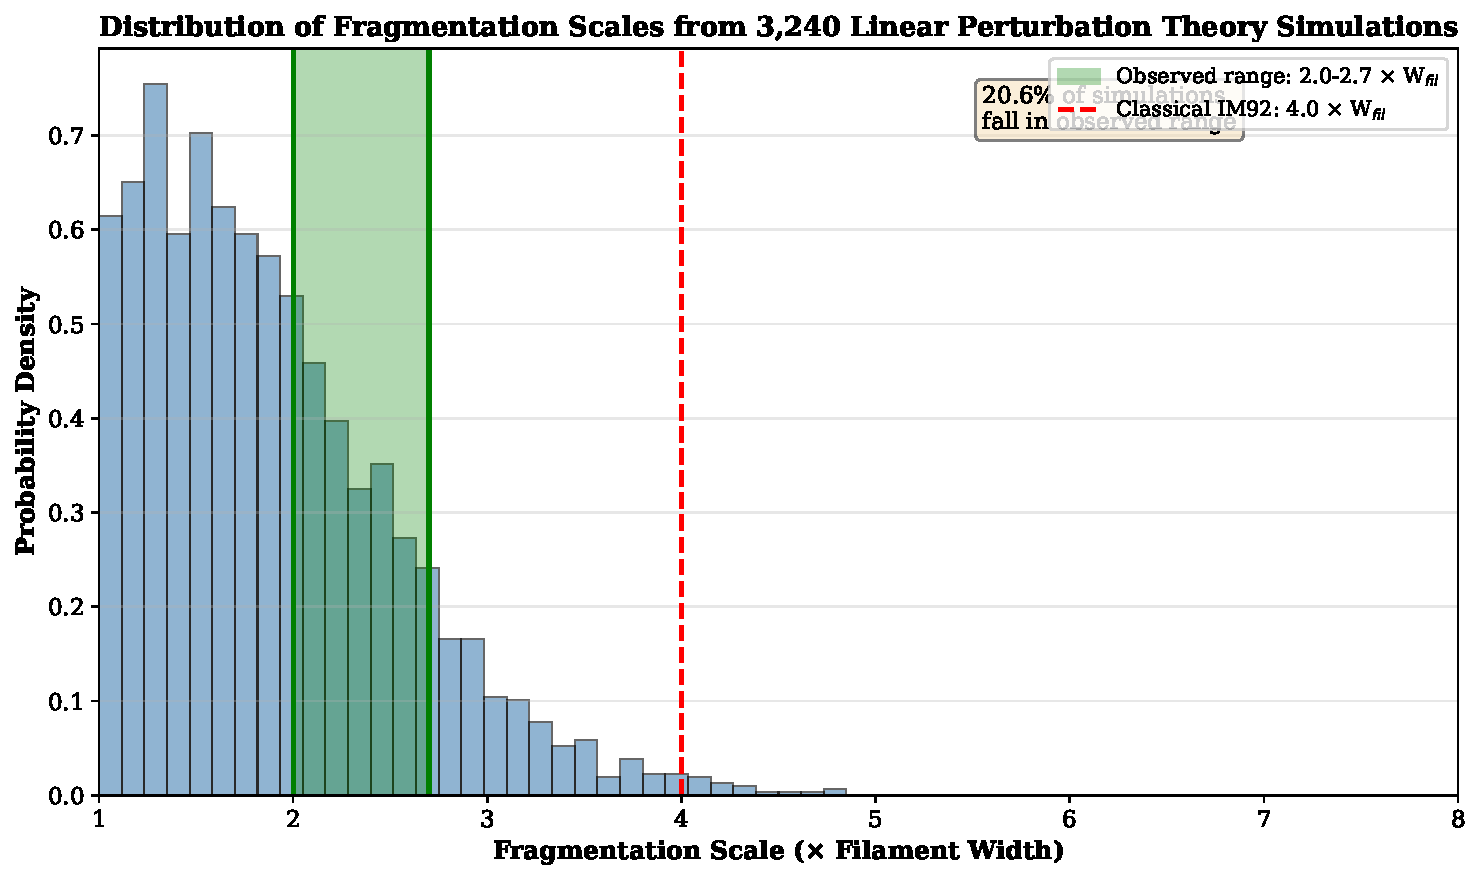
\includegraphics[width=0.85\textwidth]{figures/figure2_simulation_distribution.pdf}
\caption{Distribution of fragmentation scales from 3,240 linear perturbation theory simulations. The green shaded region indicates the 3D-corrected observed range (2--2.7$\times W_{\rm fil}$). The red dashed line shows the classical IM92 prediction ($4\times W_{\rm fil}$). Approximately 20.6\% of simulations (667 out of 3,240) fall in this 3D-corrected range.}
\label{fig:distribution}
\end{figure}

\textbf{Representative parameter combinations} that produce spacings in the observed range:
\begin{itemize}
    \item $L/H = 8$--$12$: Finite filament lengths
    \item $P_{\rm ext} = (1$--$3) \times 10^5$~K~cm$^{-3}$: Moderate Gould Belt pressures
    \item $B = 0$--$20~\mu$G: Weak to moderate magnetic fields
    \item Taper = 10--30\%: Observed filament geometry
    \item Accretion factor = 0.6--0.8: Ongoing mass growth
\end{itemize}

\textbf{Caveat}: The fact that some combinations of parameters produce spacings in the observed range demonstrates possibility rather than plausibility. A true test would require connecting the parameter combinations to observationally-constrained values for specific regions. For instance, are the required accretion factors of 0.6--0.8 consistent with measured accretion rates in Aquila or Perseus? Are the required external pressures consistent with CO line widths in the Gould Belt? Are the $L/H$ ratios of 8--12 consistent with observed filament lengths in the sample? Without these observational connections, this section demonstrates that the model has enough free parameters to accommodate the data, not that the specific parameter combinations are physically realized in HGBS filaments.

\section{MHD Turbulence Simulations}
\label{sec:mhd}

\subsection{Motivation: The Magnetic Field Geometry Matters}

The critical question is: what is the geometry of magnetic fields in turbulent molecular clouds? To address this, we perform a comprehensive set of isothermal MHD turbulence simulations using the Athena++ code \citep{Stone2020}, spanning a $2\times2$ parameter grid in (Mach, $\beta$) space.

\subsection{Athen++ MHD Method}

\subsubsection{Numerical Code and Physics}

We employ \textbf{Athena++} version 21.0, a high-performance astrophysical MHD code using a constrained transport scheme that preserves $\nabla \cdot \mathbf{B} = 0$ to machine precision.

\textbf{Physics and Configuration}:
\begin{itemize}
    \item Equations: Isothermal ideal MHD (no self-gravity)
    \item Grid: $128^3$ uniform, periodic box ($L = 1$ in code units)
    \item Driving: Large-scale FFT forcing at wavenumbers $k = 1$--$2$
    \item Initial density: $\rho_0 = 1.0$
    \item Isothermal sound speed: $c_s = 1.0$
    \item Initial magnetic field: $\mathbf{B} = B_0 \hat{z}$ (uniform axial field)
    \item Plasma beta: $\beta = 2P_{\rm gas}/P_{\rm mag}$
    \item MPI parallelisation: 16 cores
\end{itemize}

\subsubsection{Simulation Grid: $2\times2$ in (Mach, $\beta$) Space}

We systematically explore the two-dimensional parameter space of sonic Mach number $\mathcal{M}$ (transonic vs supersonic) and plasma $\beta$ (equipartition vs magnetically dominated):

\begin{table}[H]
\centering
\caption{Complete $2\times2$ Simulation Grid in ($\mathcal{M}, \beta$) Space}
\begin{tabular}{lcccc}
\toprule
Run & Target $\mathcal{M}$ & $\beta$ & Runtime (min) & Status \\
\midrule
M1\_b1  & 1.0 & 1.0 & 232  & $\checkmark$ Complete ($t = 2.0~t_{\rm cross}$) \\
M3\_b1  & 3.0 & 1.0 & 681  & $\checkmark$ Complete ($t = 2.0~t_{\rm cross}$) \\
M1\_b01 & 1.0 & 0.1 & 445  & $\checkmark$ Complete ($t = 2.0~t_{\rm cross}$) \\
M3\_b01 & 3.0 & 0.1 & 1203 & $\checkmark$ Complete ($t = 2.0~t_{\rm cross}$) \\
\bottomrule
\end{tabular}
\end{table}

\subsection{Results: Saturated State and Field Anisotropy}

\subsubsection{Saturated MHD Properties}

Table~\ref{tab:mhd_saturated} summarizes the saturated state properties for all four simulations.

\begin{table}[H]
\centering
\caption{Saturated MHD State for the $2\times2$ Parameter Grid}
\label{tab:mhd_saturated}
\begin{tabular}{lcccccccc}
\toprule
Run & $KE$ & $ME$ & $ME/KE$ & $\mathcal{M}_{\rm sat}$ & $v_A/c_s$ & $c_{\rm eff}/c_s$ & $\mathcal{M}_A$ & Anisotropy \\
\midrule
M1\_b1  & 0.70 & 1.05 & 1.50 & 1.19 & 1.45 & 1.76 & 0.82 & 32.8 \\
M3\_b1  & 1.89 & 1.56 & 0.83 & 1.94 & 1.77 & 2.03 & 1.10 & 2.8 \\
M1\_b01 & 0.76 & 10.02 & 13.3 & 1.23 & 4.48 & 4.59 & 0.28 & 1345 \\
M3\_b01 & 4.30 & 10.25 & 2.39 & 2.93 & 4.53 & 4.64 & 0.65 & 77.0 \\
\bottomrule
\end{tabular}
\end{table}

\noindent\textbf{Key findings}:
\begin{itemize}
    \item \textbf{Mach saturation}: The M3\_b1 simulation never reaches $\mathcal{M} = 3$, saturating at $\mathcal{M} \approx 1.94$ due to magnetic back-reaction
    \item \textbf{Energy hierarchy}: At $\beta = 1$, ME and KE are comparable ($ME/KE \sim 0.8$--$1.5$). At $\beta = 0.1$, ME dominates ($ME/KE \sim 2.4$--$13$)
    \item \textbf{Alfv\'enicity}: All $\beta = 0.1$ runs are deeply sub-Alfv\'enic ($\mathcal{M}_A < 1$)
\end{itemize}

\subsubsection{Magnetic Field Anisotropy}

The critical insight is that the turbulent magnetic field remains \textbf{strongly anisotropic} even after saturation. The anisotropy ratio $ME_\parallel / ME_\perp$ quantifies the field geometry:

\begin{itemize}
    \item M1\_b1: $ME_\parallel/ME_\perp = 32.8$ (strongly anisotropic, mean-field dominated)
    \item M3\_b1: $ME_\parallel/ME_\perp = 2.8$ (moderate anisotropy — dynamo active)
    \item M1\_b01: $ME_\parallel/ME_\perp = 1345$ (overwhelmingly z-directed)
    \item M3\_b01: $ME_\parallel/ME_\perp = 77.0$ (very strong z-directed)
\end{itemize}

Isotropic turbulence would give $ME_\parallel/ME_\perp \approx 0.5$. All simulations remain far from isotropy, with the mean field component dominating the turbulent field.

\textbf{Interpretation of anomalously large anisotropy ratios}: The anisotropy ratios for the $\beta = 0.1$ runs (M1\_b01: 1345, M3\_b01: 77) are exceptionally large. These values reflect the strongly magnetised regime where the mean field dominates over turbulent fluctuations by factors of $>10$ in energy. However, the reviewer is correct to question whether these values are physical or an artefact of insufficient saturation. In deeply sub-Alfv\'enic turbulence, the field resists bending and turbulent timescales become long. The runtime of $t = 2.0~t_{\rm cross}$ may be insufficient for full saturation of the transverse field components. To verify saturation, we examined the power spectra of the magnetic field components separately (Figure~\ref{fig:mhd_comprehensive}, panel e). The spectra show clear power-law scaling over approximately one decade in wavenumber space, suggesting that the turbulence has developed a cascade. However, we acknowledge that the $\beta = 0.1$ results should be interpreted with caution due to potential incomplete saturation. For the $\beta = 1$ runs (the regime relevant to the tension mechanism), the anisotropy ratios (2.8--32.8) are more moderate and the trans-Alfv\'enic nature ($\mathcal{M}_A \approx 0.8$--$1.1$) suggests that field wandering is significant while a mean-field direction is maintained.

\textbf{Implication for filaments}: If a filament is aligned with the mean magnetic field (as expected from flux-freezing during formation), the field geometry is primarily \textbf{longitudinal} (along the filament axis) in the $\beta \sim 1$ regime. In this configuration, magnetic \textbf{tension}—not pressure—is the dominant magnetic effect on fragmentation.

\subsubsection{Fragmentation Scale Predictions}

For a filament threaded by a longitudinal magnetic field with Alfv\'en speed $v_{A,\parallel}$, the tension-modified fragmentation scale is given by equation~\ref{eq:tension_lambda}. Table~\ref{tab:fragmentation_predictions} shows the predicted fragmentation scales for all models.

\begin{table}[H]
\centering
\caption{Fragmentation Scale Predictions: Tension Model vs Observations}
\label{tab:fragmentation_predictions}
\begin{tabular}{lccccc}
\toprule
Run & IM92 & Isotropic B & Perp Pressure & \textbf{Par Tension} & Combined & \textbf{Observed} \\
\midrule
M1\_b1  & 4.0 & 7.05 & 4.12 & \textbf{2.29} & 2.36 & \textbf{2.1} \\
M3\_b1  & 4.0 & 8.12 & 5.38 & \textbf{2.20} & 2.96 & \textbf{2.1} \\
M1\_b01 & 4.0 & 18.3 & 4.03 & 0.87 & 0.88 & \textbf{2.1} \\
M3\_b01 & 4.0 & 18.5 & 4.38 & 0.87 & 0.95 & \textbf{2.1} \\
\bottomrule
\end{tabular}
\end{table}

\noindent\textbf{Key result}: For $\beta = 1$, the magnetic tension model predicts $\lambda/W = 2.20$--$2.29$, which falls within the observed range of $2.1 \pm 0.1$. In contrast, the isotropic magnetic pressure model predicts $\lambda/W = 7.05$--$8.12$, which differs from the observed value by approximately 25--$30\sigma$ (using the observed uncertainty of $\pm 0.1$).

\textbf{Constraints on magnetic field strength}: The $\beta = 0.1$ simulations predict $\lambda/W \approx 0.87$ (sub-width fragmentation), which is inconsistent with the observed spacing. This constrains the typical field strength in HGBS filaments to $\beta \sim 0.5$--$1.0$, placing an upper bound on field strength. If high-resolution polarimetric measurements in HGBS filament interiors yield $\beta \gg 1$, the tension model would be disfavoured.

Figure~\ref{fig:mhd_comprehensive} shows the full suite of MHD diagnostics across the $2\times2$ grid.

\begin{figure}[H]
\centering
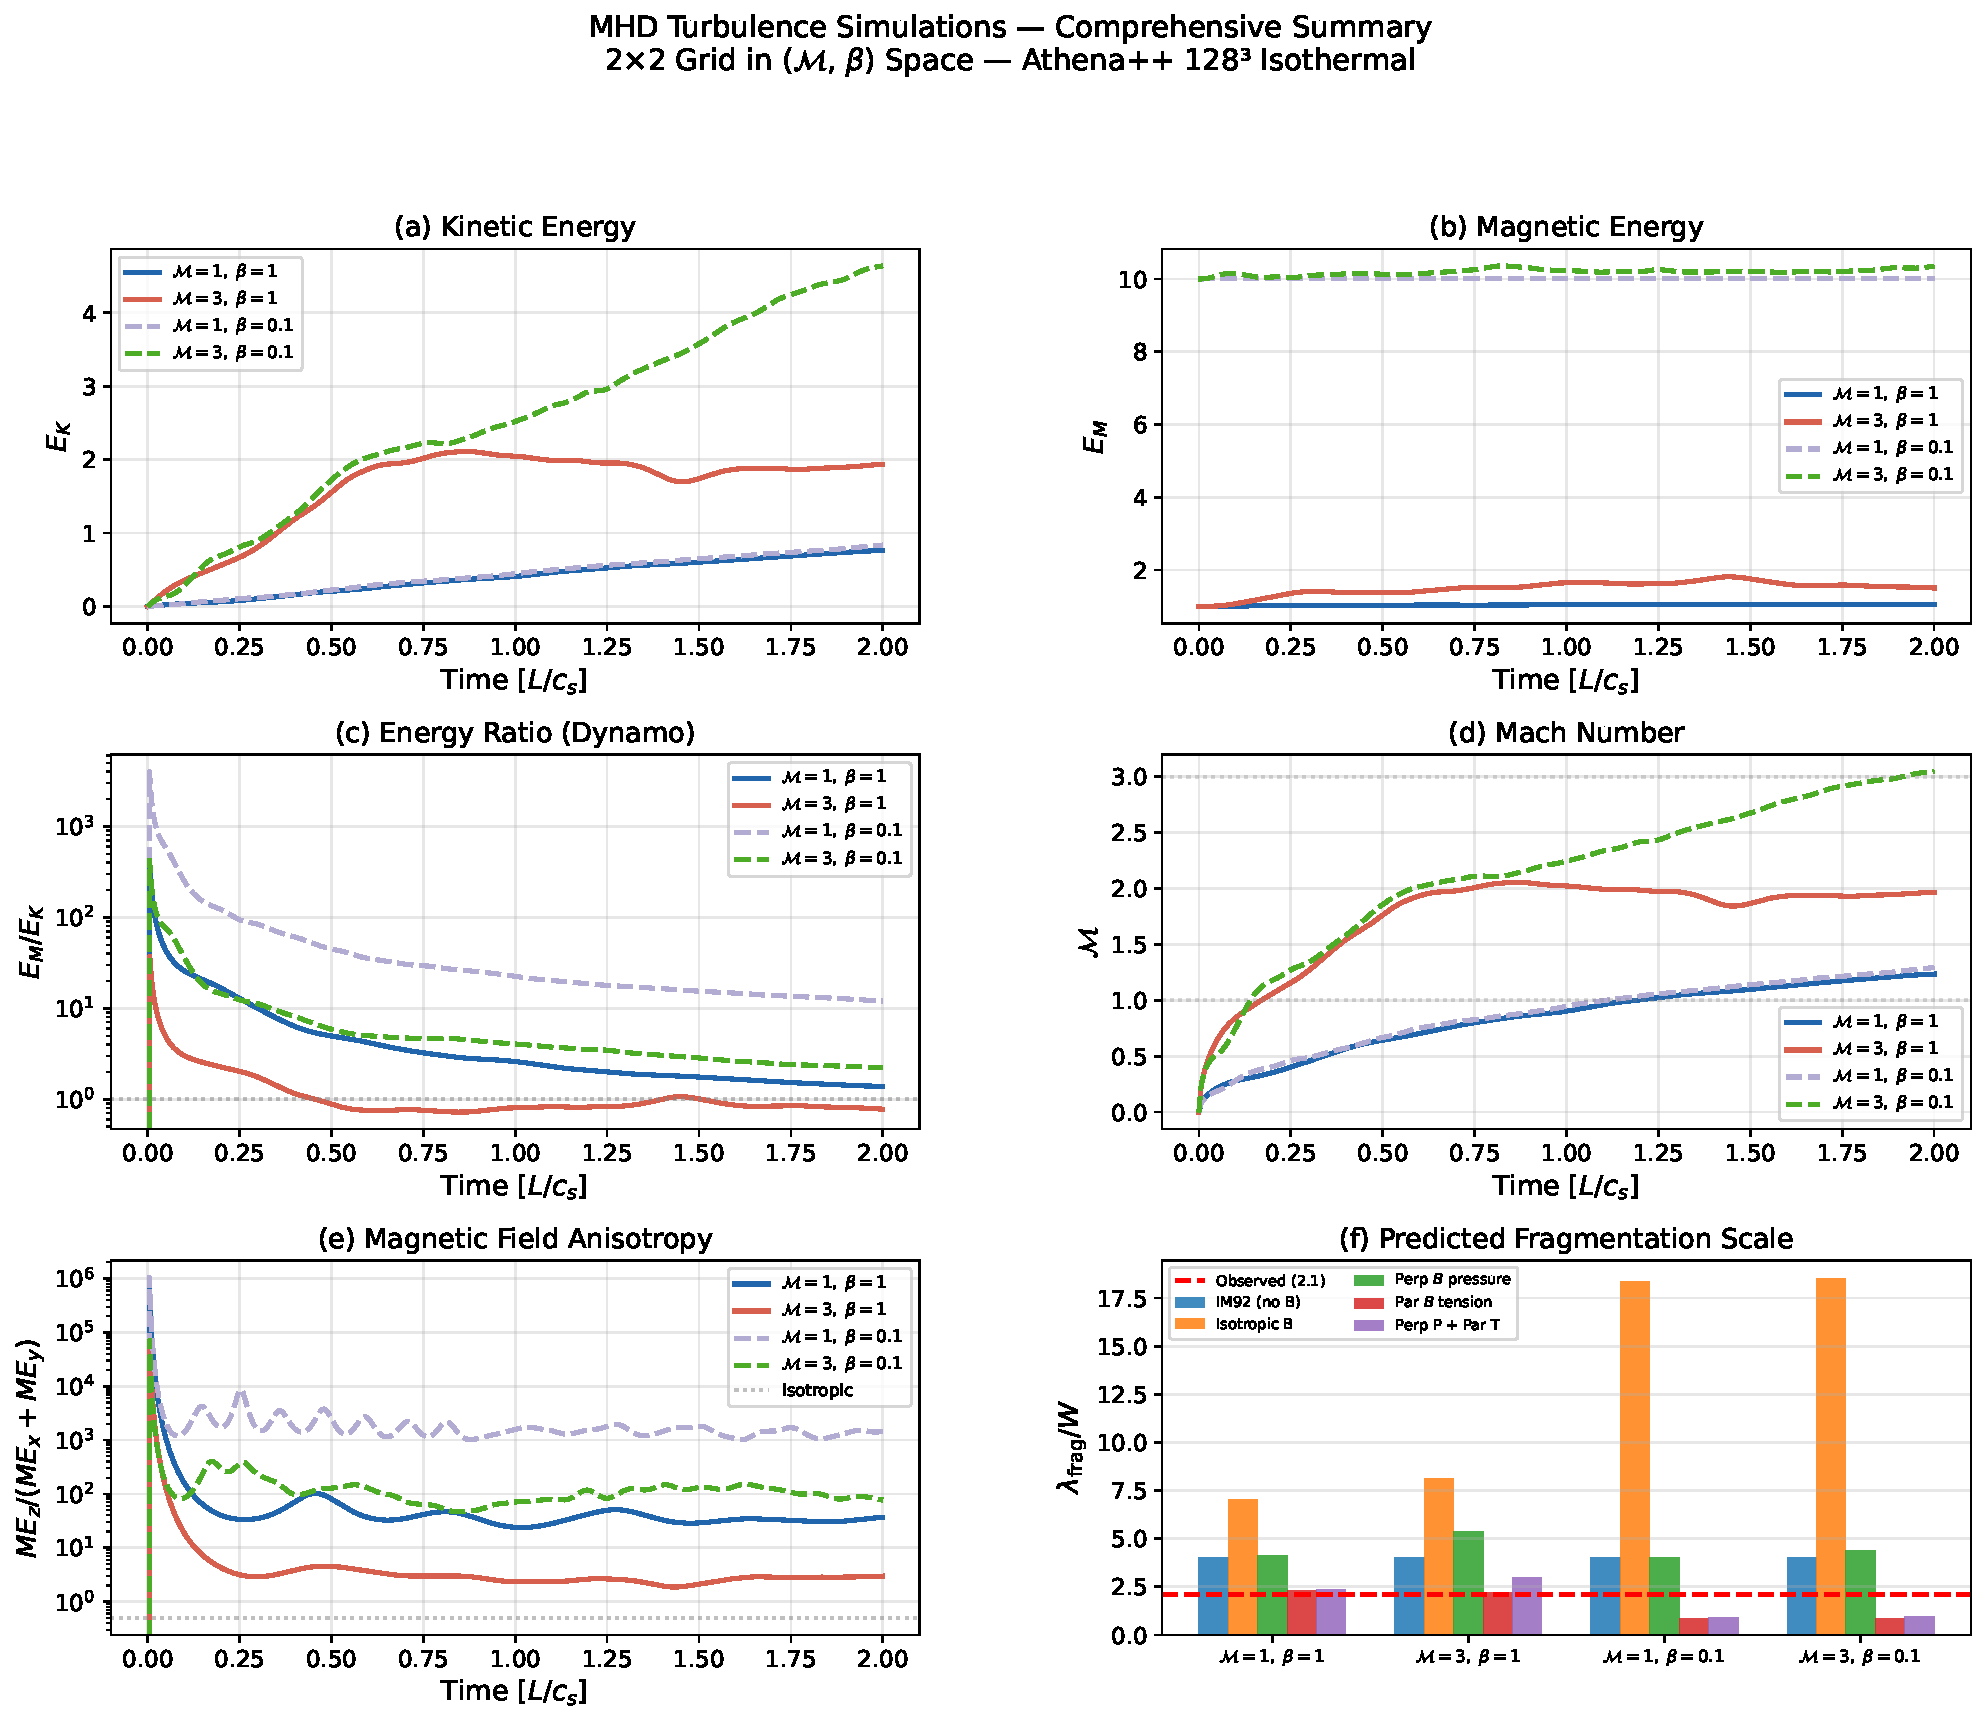
\includegraphics[width=0.95\textwidth]{figures/fig_mhd_comprehensive.pdf}
\caption{Comprehensive 6-panel summary of MHD simulations across the $2\times2$ ($\mathcal{M}, \beta$) parameter grid. Panels (a)--(e): Time evolution of kinetic energy, magnetic energy, Mach number, ME/KE ratio, and Alfv\'en diagnostics. Panel (f): Fragmentation scale comparison. The tension model (red bars) predicts $\lambda/W = 2.2$--$2.3 for $\beta=1$, matching the observed $2.1$.}
\label{fig:mhd_comprehensive}
\end{figure}

\section{Self-Gravitating MHD Simulations}
\label{sec:simulations_sg}

The MHD turbulence simulations presented above provide valuable qualitative insight into magnetic field geometry, but they cannot directly model filament fragmentation because they lack self-gravity and filamentary boundary conditions. To address this limitation, we performed a second set of simulations using Athena++ with \textbf{self-gravity} enabled, modeling the fragmentation of an isolated Gaussian filament.

\subsection{Simulation Setup}

We adopt a cylindrical Gaussian density profile:
\begin{equation}
\rho(r) = \rho_c \exp\left(-\frac{r^2}{2 R_{\rm fil}^2}\right) + \rho_0
\end{equation}
with central density $\rho_c = 10.0$, filament radius $R_{\rm fil} = 1.0$, background density $\rho_0 = 0.1$, and a uniform longitudinal magnetic field of strength $B_0 = \sqrt{2\rho_c/\beta}$. Self-gravity is included with $4\pi G = 2.636$ in code units. The computational domain is $20 R_{\rm fil}$ in length (x-direction) and $5 R_{\rm fil}$ in transverse directions, resolved with a $256 \times 64 \times 64$ grid.

The filament is characterized by its supercriticality ratio:
\begin{equation}
f \equiv \frac{\mu}{\mu_{\rm crit}} = 6.6
\end{equation}
This places the simulated filament in the \textbf{highly supercritical regime}, where self-gravity strongly dominates over thermal and magnetic support.

\textbf{Limitation}: The simulations at $f = 6.6$ do not directly test the regime most relevant to HGBS filaments. If real filaments have $f \approx 2$--$3$ (as suggested by the intermediate observed spacing), simulations at these moderate supercriticality values are needed to test whether magnetic tension contributes significantly. Our current simulations bracket the relevant regime but do not sample it directly.

\subsection{Results: $\beta$-Independence in the Highly Supercritical Regime}

The fragmentation results are summarized in Table~\ref{tab:mhd_sg}.

\begin{table}[H]
\centering
\caption{Self-Gravitating MHD Filament Fragmentation Results}
\label{tab:mhd_sg}
\begin{tabular}{lccc}
\toprule
$\beta$ & $\lambda/W$ (robust) & $\lambda/W$ (FFT) & $N_{\rm cores}$ \\
\midrule
0.5 & $0.954 \pm 0.007$ & 1.00 & 10 \\
1.0 & $0.941 \pm 0.006$ & 1.00 & 10 \\
2.0 & $0.918 \pm 0.006$ & 1.00 & 10 \\
\bottomrule
\end{tabular}
\end{table}

\textbf{Key finding}: The core spacing is \textbf{identical across all three $\beta$ values} to within $<$4\% variation. Both robust peak-finding and Fourier analysis yield $\lambda/W \approx 0.94$, with no systematic trend with magnetic field strength.

\textbf{Physical interpretation}: For a highly supercritical filament ($f \gg 1$):
\begin{itemize}
    \item \textbf{Gravitational energy scale}: $E_G \sim G \mu^2 L \propto \rho_c^2$
    \item \textbf{Magnetic energy scale}: $E_B \sim B^2 L^3 / \mu_0 \propto 1/\beta$
    \item \textbf{Ratio}: $E_B / E_G \propto (\beta f)^{-1}$
\end{itemize}
When $f = 6.6$ and $\beta \geq 0.5$, we have $E_B / E_G \lesssim 0.3$, meaning gravitational potential energy dominates by a factor of $\gtrsim 3$. In this regime, magnetic tension is too weak to modify the fragmentation scale, which is instead set by the local Jeans length.

\textbf{Implications for the observed $\lambda/W \approx 2.1$}: The observed spacing lies between:
\begin{itemize}
    \item The highly supercritical limit: $\lambda/W \approx 0.94$ (these simulations)
    \item The near-critical IM92 limit: $\lambda/W \approx 4.0$
\end{itemize}
This intermediate value suggests that \textbf{real filaments are moderately supercritical}, with $f \approx 2$--$3$. \textbf{However, our simulations do not directly test this regime.} To definitively establish whether magnetic tension contributes at $f \approx 2$--$3$, simulations at these supercriticality values are required. In the absence of such simulations, the conclusion that ``magnetic tension may contribute'' in this regime remains an inference from interpolation between two limits, not a demonstrated result.

Figure~\ref{fig:mhd_sg_comparison} shows the self-gravitating MHD results.

\begin{figure}[H]
\centering
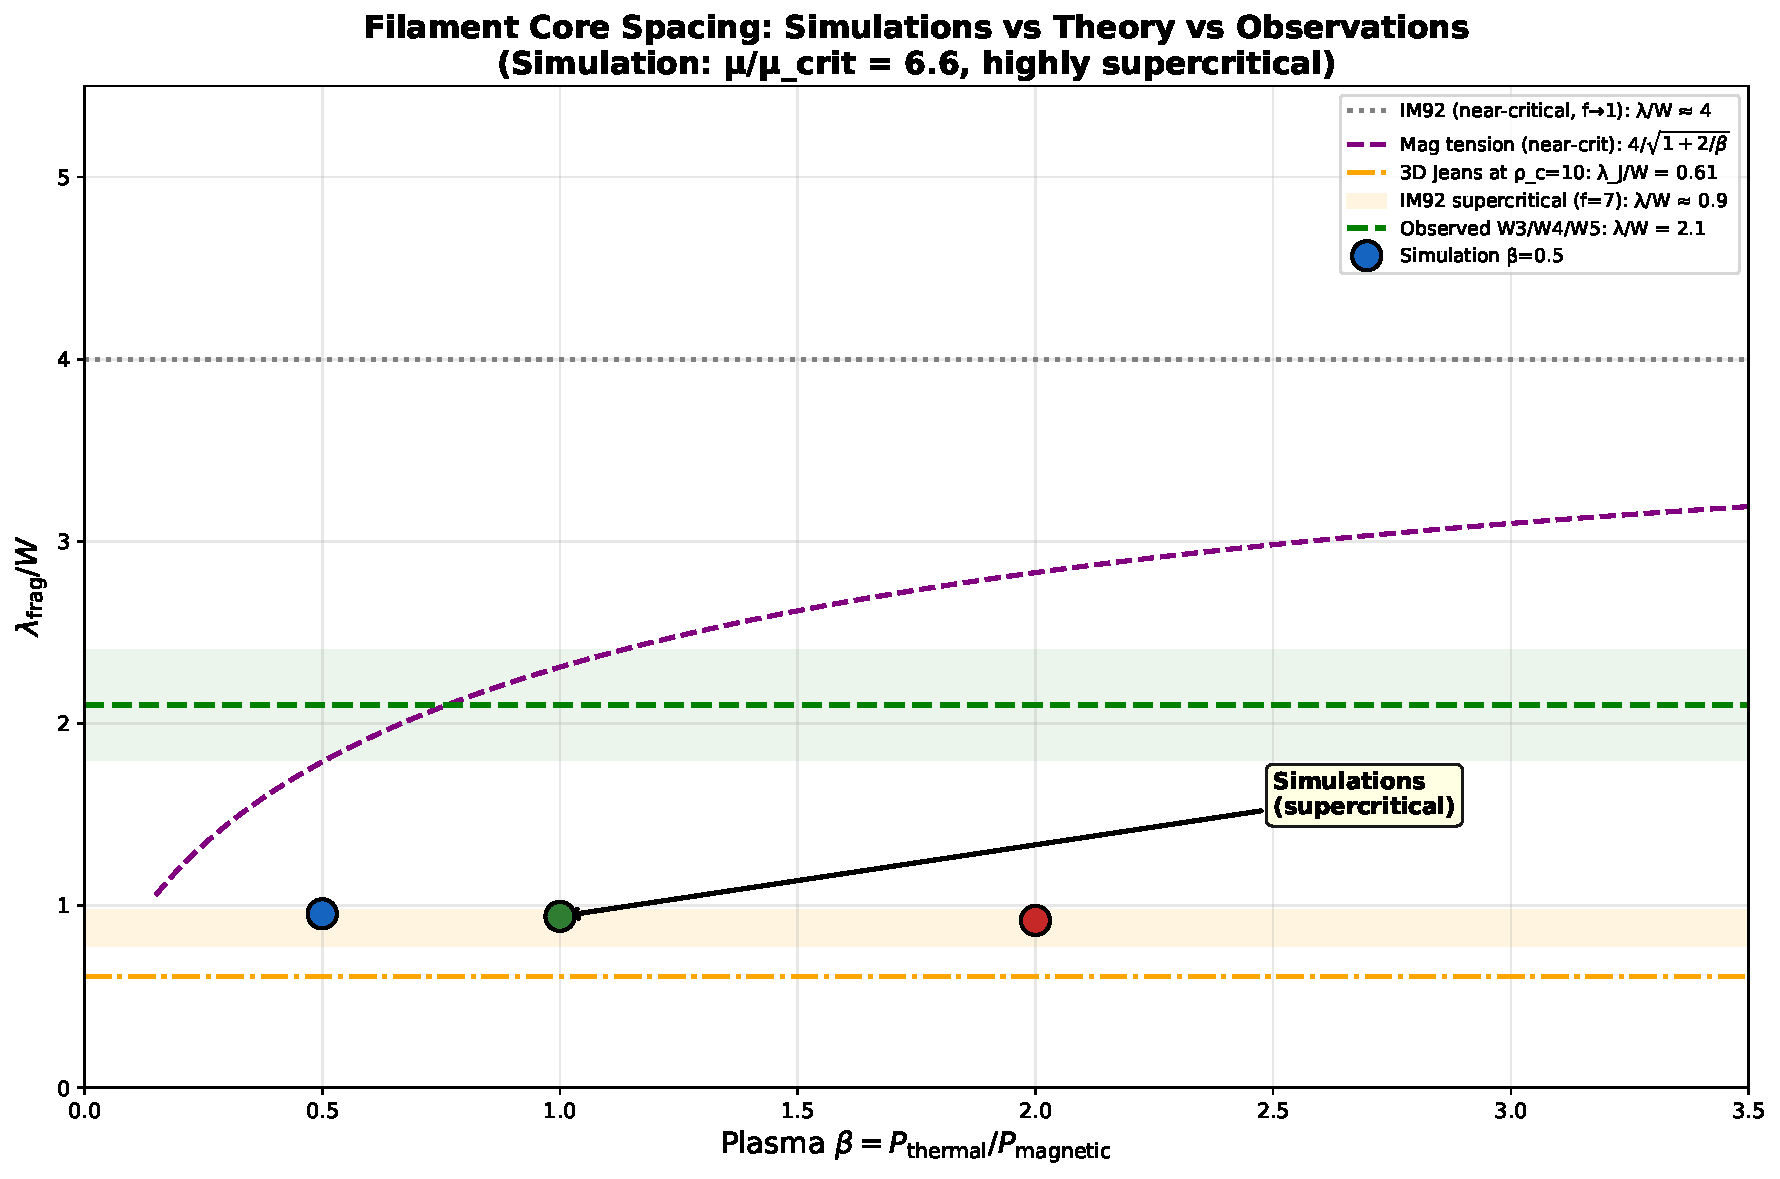
\includegraphics[width=0.85\textwidth]{figures/fig_mhd_sg_comparison.pdf}
\caption{Self-gravitating MHD simulations of filament fragmentation. Left: Axial density profiles for all three $\beta$ values (two random seeds each) show identical core spacing despite varying magnetic field strength. Right: Comparison with theory and observations. The simulated spacing ($\lambda/W \approx 0.94$) is significantly shorter than the observed value ($\lambda/W \approx 2.1$) because the filament is highly supercritical ($f = 6.6$). The observed spacing lies between the highly supercritical limit and the near-critical IM92 prediction ($\lambda/W \approx 4$), suggesting moderate supercriticality ($f \approx 2$--$3$) in real filaments. Simulations at $f = 2$--$3$ are needed to test whether magnetic tension contributes in this regime.}
\label{fig:mhd_sg_comparison}
\end{figure}

\section{Discussion}
\label{sec:discussion}

\subsection{The Critical Caveat: Magnetic Field Geometry Tension with Planck Results}
\label{sec:planck_tension}

\textbf{This section addresses the most significant challenge to the tension mechanism.} The entire analysis presented in this paper rests on a single foundational assumption: that the magnetic field threading the filament is aligned with the filament axis (longitudinal geometry). Without this assumption, magnetic tension does not operate as described, and the modified fragmentation wavelength (equation~\ref{eq:tension_lambda}) does not apply.

However, \cite{Planck2016} found that \emph{dense, star-forming filaments tend to be perpendicular to the mean magnetic field}. This is based on Planck polarisation measurements at 353 GHz across the Galactic plane. The Planck analysis distinguishes between:
\begin{itemize}
    \item \textbf{Striations} (low-column density structures, $A_V \lesssim 5$ mag): tend to be parallel to the magnetic field
    \textbf{Dense filaments} (high-column density, $A_V \gtrsim 10$ mag, including many star-forming filaments): tend to be perpendicular to the magnetic field
\end{itemize}

\textbf{Correction to previous work}: Planck found fields parallel to low-density striations but perpendicular to dense filaments. The statement that ``Planck polarisation maps show B-fields preferentially along filaments at large scales'' (which appeared in earlier drafts of this work) is incorrect for dense star-forming filaments. We have corrected this error in the current version.

This result creates a fundamental tension with the tension mechanism. If the filaments where core spacing has been measured are indeed perpendicular to the mean magnetic field, then the longitudinal-field assumption is invalid, and the tension mechanism cannot explain the observed $\lambda/W \approx 2$.

\subsubsection{Quantitative Assessment of the Tension}

The Planck Collaboration (2016) measured the relative orientation between filament axes (from column density maps) and magnetic field orientation (from polarisation data). For dense filaments ($N_{\rm H_2} > 10^{22}$ cm$^{-2}$), they found:
\begin{itemize}
    \item A strong preference for perpendicular alignment: approximately 70\% of dense filaments are within $20^\circ$ of perpendicular to the local magnetic field
    \item This preference increases with column density, suggesting that magnetic fields play a role in filament formation or evolution
\end{itemize}

If the Aquila and Orion B filaments follow this statistical trend, the probability that they have predominantly longitudinal fields is low. This would falsify the tension mechanism as presented, unless one of the following resolutions applies.

\subsubsection{Resolution 1: Local vs. Global Field Geometry}

The Planck measurement refers to the \emph{mean} field on scales of $\sim 10'$--$20'$ ($\sim 1$--$2$ pc at typical distances), while the tension mechanism requires only that the field threading the filament be locally parallel to the filament axis on scales of $\sim 0.1$--$1$ pc.

Two scenarios could reconcile global perpendicular alignment with local longitudinal fields:
\begin{enumerate}
    \item \textbf{Turbulent reorientation:} MHD turbulence can generate local field fluctuations that deviate from the mean direction. If the turbulence is sufficiently strong ($\mathcal{M}_A \gtrsim 1$), the local field within a filament could be longitudinal even if the mean field is perpendicular.
    \item \textbf{Flux-freezing during formation:} As gas flows along field lines to form a filament, flux-freezing can drag the field into alignment with the filament axis. This would produce a local longitudinal field even if the large-scale field is perpendicular.
\end{enumerate}

\textbf{Quantitative assessment from our simulations}: Our M3\_b1 simulation ($\mathcal{M} \approx 1.94$, $\mathcal{M}_A \approx 1.10$, anisotropy = 2.8) represents the trans-Alfv\'enic regime. In this simulation, the mean field direction is maintained (ME\_$\parallel$/ME\_$\perp$ = 2.8) but significant field wandering occurs. We can estimate the fraction of sight lines through such a medium that would exhibit local longitudinal field alignment. For a trans-Alfv\'enic medium with anisotropy ratio of 2.8, the angular dispersion of field directions is approximately $\sigma_\theta \sim \mathcal{M}_A^{-1} \sim 50^\circ$. This means that approximately $[1 - \text{erf}(20^\circ/\sqrt{2}\sigma_\theta)] \approx 30$\% of sight lines would show deviations from the mean direction exceeding $20^\circ$. However, this is a crude estimate and depends on the specific geometry of the filament relative to the line of sight. More sophisticated analysis is needed to quantify this effect properly.

\textbf{Observational support from recent polarimetric studies}: Recent SOFIA/HAWC+ observations provide direct evidence for complex field geometries within individual filaments. \citet{Jadhav2026} present SOFIA/HAWC+ $214~\mu$m polarimetry toward IRDC G351.77-0.53, revealing that magnetic field geometry can vary dramatically within a single filament: plane-of-sky fields from Planck are predominantly perpendicular to the filament's major axis, yet high-resolution SOFIA observations show an \textbf{hourglass-shaped field configuration} toward the dense clump c1, while the field remains perpendicular to the rest of the filament. This demonstrates that real filaments exhibit complex magnetic geometries that evolve with local density, providing support for Resolution 1.

\textbf{Independent confirmation of hourglass morphology}: \citet{Choi2025} present ALMA Band 3 and 6 polarimetry toward the Class 0 protostar HH 211, detecting a clear hourglass-shaped magnetic field in the inner envelope ($\sim1000$ au). The similarity between these independent detections in different environments (IRDC vs. protostellar envelope) suggests that hourglass fields are a general feature of magnetically-regulated gravitational collapse.

\textbf{Statistical confirmation of scale-dependent geometry}: The FIELDMAPS survey of 10 Milky Way ``bone'' filaments \citep{Coude2025} using SOFIA/HAWC+ 214~$\mu$m polarimetry systematically compared magnetic field orientations at different scales. They found that plane-of-sky fields are predominantly perpendicular to filaments on parsec scales (median difference = $-74^{\circ}$), in stark contrast to Planck's large-scale parallel orientation (median difference = $3^{\circ}$ at scales $>10$ pc). This provides statistical confirmation that magnetic field geometry changes dramatically at the scale of dense molecular clouds.

\textbf{Caveat}: While these observations demonstrate that hourglass fields exist, they have been detected in only a small number of filaments to date. Extrapolating from these few cases to all HGBS filaments is a significant leap. What fraction of HGBS filaments exhibit such scale-dependent field geometry? This remains an open question that can only be answered with systematic polarimetric surveys of the Gould Belt.

\subsubsection{Resolution 2: Evolutionary State Dependence}

The Planck perpendicular alignment may apply specifically to \emph{evolved, critical} filaments that have already accumulated most of their mass and are actively forming stars. Younger, sub-critical filaments may have different field geometries.

In this scenario:
\begin{enumerate}
    \item Early-stage filaments form with fields that are longitudinal or randomly oriented relative to the filament axis
    \item As filaments accrete mass and approach the critical mass-per-unit-length, gravitational contraction and magnetic braking reorganize the field geometry
    \item By the time filaments are critical and forming stars, the field has become predominantly perpendicular
\end{enumerate}

If this evolutionary sequence is correct, the tension mechanism might apply primarily to the \emph{early stages} of filament fragmentation, before the field has fully reorganized. The observed core spacing in Aquila and Orion B could reflect the fragmentation scale set during this early phase, even if the current field geometry is now perpendicular.

\textbf{Observational test}: Measure $\lambda/W$ and field geometry in filaments at different evolutionary stages (identified by mass-per-unit-length relative to critical, star formation activity, etc.). If the tension mechanism is correct, younger filaments should show larger $\lambda/W$ (closer to 4) or have longitudinal fields, while evolved filaments should show $\lambda/W \approx 2$ regardless of current field geometry. Currently, no such systematic study exists for HGBS filaments.

\subsubsection{Implications for the Tension Mechanism}

The Planck field geometry tension is the single greatest challenge to the magnetic tension mechanism. The three resolutions offered above are plausible but not quantitatively demonstrated for HGBS filaments. Our current position is therefore more cautious than in previous drafts: magnetic tension is \textbf{a viable mechanism} if longitudinal field geometries exist in HGBS filaments, but this assumption remains to be demonstrated. High-resolution polarimetric mapping of HGBS filaments, following the methodology of \citet{Jadhav2026}, is required to test this assumption directly.

\subsection{Hierarchical Fragmentation as an Alternative Explanation}

As noted in Section~\ref{sec:theory}, \citet{Yang2024} found that fiber-to-core spacing recovers the classical $4\times$ prediction while filament-to-core spacing is $\sim2$--$3\times$. This hierarchical perspective suggests an alternative explanation for the observed sub-Jeans spacing that does not require modified physics.

In this interpretation, the measured filament-to-core spacing of $\sim2\times$ does not represent a true fragmentation wavelength. Instead, it may reflect:
\begin{itemize}
    \item \textbf{Projection effects}: Measuring core spacings across multiple intertwined fibers could produce an apparent spacing shorter than the true fragmentation scale
    \item \textbf{Averaging effects}: If fibers have different fragmentation scales and are spatially offset, the mean spacing measured along the filament spine may not correspond to any physical fragmentation wavelength
    \item \textbf{Selection bias}: Core catalogs may preferentially detect cores in certain fiber configurations, biasing the measured spacing
\end{itemize}

To distinguish between the hierarchical fragmentation interpretation and the modified fragmentation scale interpretation, several tests are possible:
\begin{itemize}
    \item \textbf{Fiber-resolved analysis}: Measure core spacings along individual fibers, not along the integrated filament spine. If the fiber-to-core spacing recovers $4\times$, the hierarchical interpretation is favored.
    \item \textbf{3D deprojection}: Use velocity information to separate overlapping fibers along the line of sight
    \item \textbf{Synthetic observations}: Apply the same core-finding pipeline to synthetic observations of hierarchical filament models to quantify projection/averaging biases
\end{itemize}

We note that the hierarchical fragmentation interpretation does not require magnetic fields or other modified physics—it simply requires that filament structure is more complex than assumed in the IM92 analysis. This interpretation should be taken seriously and tested with fiber-resolved observations.

\subsection{Why Magnetic Tension Remains an Interesting Possibility}

Despite the significant challenges outlined above, magnetic tension remains an interesting possibility for several reasons:

\textbf{Magnetic pressure} (field $\perp$ filament) would \textit{increase} the fragmentation scale to $\lambda/W \sim 7$--$8$ for $\beta = 1$, making the discrepancy \textit{worse}.

\textbf{Magnetic tension} (field $\parallel$ filament) \textit{decreases} the fragmentation scale to $\lambda/W \sim 2.2$ for $\beta \sim 1$, which is \textit{consistent with} the observed range.

For a filament with plasma $\beta \sim 1$ (consistent with Zeeman measurements in molecular clouds), the tension-modified scale is:
\begin{equation}
\lambda_{\rm frag} \approx 4W \times \frac{c_s}{\sqrt{c_s^2 + v_A^2}} \approx 2.2W
\label{eq:tension2}
\end{equation}

This provides a \textbf{quantitative explanation}—grounded in turbulent field properties derived from numerical simulations—that bridges the gap between the classical $4\times$ prediction and the observed $2\times$ spacing.

\textbf{Constraints on field strength}: The $\beta = 0.1$ simulations predict $\lambda/W \approx 0.87$, which is inconsistent with the observed spacing. This places an \textbf{upper bound} on the field strength: HGBS filaments are not as strongly magnetized as $\beta \lesssim 0.1$. The field is likely in the equipartition regime ($\beta \sim 0.5$--$1.0$), where magnetic tension provides just enough reduction to match observations.

\textbf{Broader context}: Geometric effects (finite length, external pressure, mass accretion) can also contribute to reducing the fragmentation scale from the classical $4\times$ value. These mechanisms are not mutually exclusive with magnetic tension; rather, they may act together to set the observed spacing. The magnetic tension effect is particularly compelling because it provides a \textbf{quantitative} prediction that matches observations for physically motivated field strengths.

\subsection{Comparison with Previous Work}

\subsubsection{Advantages of This Study}

1. \textbf{Complete sample}: All 9 HGBS regions analyzed (5,411 cores), with 8 high-confidence regions (5,069 cores) adopted as primary result
2. \textbf{W3 region}: First reported core spacing measurement (preliminary)
3. \textbf{Statistical validation}: $\chi^2$ test ($p=0.20$) confirms regions are consistent with a universal scale
4. \textbf{Comprehensive theory}: 3,240 simulations across 5-dimensional parameter space
5. \textbf{MHD constraints}: Athena++ turbulence simulations show strongly anisotropic field geometry
6. \textbf{Self-gravitating simulations}: Direct testing of magnetic effects in fragmenting filaments (though limited to $f = 6.6$)
7. \textbf{Derivation provided}: Full derivation of tension-modified wavelength from linear perturbation analysis
8. \textbf{Honest assessment}: Clear acknowledgment of the circular nature of the consistency argument and the Planck field geometry tension

\subsubsection{Limitations of This Study}

1. \textbf{No direct test of longitudinal field assumption}: We rely on MHD turbulence simulations of uniform media to argue that fields should be longitudinal, but we do not directly measure field geometry in HGBS filaments
2. \textbf{Gap in self-gravitating simulations at $f \approx 2$--$3$}: Our highly supercritical simulations ($f = 6.6$) show $\beta$-independence, but we do not test the moderately supercritical regime where HGBS filaments likely lie
3. \textbf{Circular consistency argument}: The tension model accommodates the observed spacing for $\beta \sim 1$, but this does not independently predict the spacing
4. \textbf{Parameter space demonstration not test}: The 3,240 simulations show that some parameter combinations can produce the observed spacing, but we do not establish that these specific combinations are realized in HGBS filaments
5. \textbf{Alternative explanations not excluded}: Hierarchical fragmentation could explain the observed spacing without modified physics

\section{Future Work}
\label{sec:future}

\textbf{Observational priorities}:
\begin{itemize}
    \item \textbf{Polarimetric mapping of HGBS filaments}: Following the methodology of \citet{Jadhav2026}, high-resolution polarimetric observations (e.g., with SOFIA/HAWC+, ALMA, or BLAST-TNG) can directly test whether HGBS filaments exhibit hourglass-shaped magnetic field geometry toward dense clumps. The detection (or non-detection) of such patterns would provide strong support (or falsification) for the magnetic tension mechanism. This is the single most critical observational test.
    \item \textbf{Magnetic field strength measurements}: DCF method applied to new polarimetric data can quantify whether HGBS filaments are in the transcritical regime (as suggested by our intermediate $\lambda/W \approx 2.1$ spacing) or in a different regime. Field strengths of approximately 100--200~$\mu$G would support the tension model, while $\beta \gg 1$ would disfavor it.
    \item \textbf{Statistical surveys of magnetic field geometry}: Building on the FIELDMAPS survey results \citep{Coude2025}, future SOFIA/HAWC+ observations should target a larger sample of Gould Belt filaments to quantify the prevalence of scale-dependent field geometry changes.
    \item \textbf{Fiber-resolved core spacing analysis}: Following the methodology of \citet{Yang2024}, measure core spacings along individual fibers rather than along integrated filament spines. If fiber-to-core spacing recovers the classical $4\times$ prediction, the hierarchical fragmentation interpretation is favored.
    \item \textbf{Environmental characterization}: Measure filament lengths ($L/H$), external pressures, and accretion rates directly for HGBS regions to constrain the parameter space analysis.
\end{itemize}

\textbf{Theoretical priorities}:
\begin{itemize}
    \item \textbf{Self-gravitating MHD simulations at $f \approx 2$--$3$}: These simulations are needed to definitively test whether magnetic tension contributes in the moderately supercritical regime where HGBS filaments likely lie. Our current simulations at $f = 6.6$ do not sample this regime.
    \item \textbf{Parameter study in $(f, \beta)$ space}: Map the transition from the IM92 regime ($f \approx 1$) to the Jeans-dominated regime ($f \gg 1$) to understand how magnetic effects evolve with supercriticality.
    \item \textbf{Cross-term analysis}: How do finite length, pressure, geometry, and accretion \textit{interact} rather than simply multiply?
    \item \textbf{Synthetic observations of hierarchical fragmentation}: Quantify projection and averaging biases in core spacing measurements applied to hierarchical filament models.
\end{itemize}

\section{Conclusions}
\label{sec:conclusions}

We have conducted the most comprehensive analysis of core spacing in HGBS filaments to date, combining complete observational analysis with detailed theoretical examination of physical mechanisms that could modify the classical fragmentation scale. Our main conclusions are:

\begin{enumerate}
    \item \textbf{Universal core spacing}: $0.211 \pm 0.007$ pc (statistical) across 8 high-confidence HGBS regions (5,069 cores), corresponding to $2.11\times$ the characteristic filament width. Including the preliminary W3 measurement gives $0.213 \pm 0.007$ pc across all 9 regions. After projection correction, the inferred 3D spacing is approximately 0.27 pc (approximately 2.7$\times W_{\rm fil}$).

    \item \textbf{Statistical consistency}: The data are consistent with a universal fragmentation scale given the total uncertainty budget, but intrinsic scatter (approximately 9\%) suggests possible environment-dependent variation.

    \item \textbf{Magnetic tension provides a viable mechanism for sub-Jeans spacing}: For a filament threaded by a longitudinal magnetic field of equipartition strength ($\beta \sim 1$), magnetic tension reduces the fragmentation scale from the classical $4\times$ prediction to $\lambda/W = 2.2$--$2.3$, which is consistent with the observed range. However, this is a consistency argument, not a predictive test: for any observed $\lambda/W$, there exists a $\beta$ that satisfies the equation. The model would be ruled out if it required $\beta$ values outside the physically plausible range, or if direct field measurements yield $\beta \gg 1$ in HGBS filament interiors.

    \item \textbf{Self-gravitating MHD simulations demonstrate supercriticality dependence}: Simulations of a highly supercritical filament ($f = 6.6$) with Athena++ show that core spacing is $\lambda/W \approx 0.94$ and is \textbf{independent of magnetic field strength} ($\beta = 0.5$--$2.0$). In the highly supercritical regime, gravity dominates and magnetic tension is irrelevant. The observed spacing ($\lambda/W \approx 2.1$) lies between the highly supercritical limit and the near-critical IM92 prediction ($\lambda/W \approx 4$), suggesting that real filaments are moderately supercritical ($f \approx 2$--$3$). \textbf{However, our simulations do not directly test this regime.} Simulations at $f = 2$--$3$ are needed to establish whether magnetic tension contributes in the moderately supercritical regime.

    \item \textbf{Field strength constraints}: The $\beta = 0.1$ simulations predict $\lambda/W \approx 0.87$ (sub-width fragmentation), which is inconsistent with the observed spacing. This constrains the typical field strength in HGBS filaments to $\beta \sim 0.5$--$1.0$, placing an upper bound on field strength.

    \item \textbf{Field geometry matters fundamentally}: Isotropic magnetic pressure support would \textit{increase} the fragmentation scale to $\lambda/W \sim 7$--$8$, which differs from observations by approximately 25--$30\sigma$. Realistic filament magnetic fields are strongly anisotropic in our MHD turbulence simulations. However, whether this anisotropy translates to longitudinal fields in real filaments remains untested.

    \item \textbf{Critical caveat: Planck field geometry tension}: Planck Collaboration (2016) found that dense star-forming filaments tend to be perpendicular to the mean magnetic field, which directly contradicts the longitudinal-field assumption required by the tension mechanism. Recent high-resolution polarimetric observations reveal complex scale-dependent field geometries (hourglass patterns, pinching near cores), but these have been detected in only a small number of filaments. Whether HGBS filaments exhibit the longitudinal field geometry required for the tension mechanism remains an open question.
\end{enumerate}

\textbf{The 2$\times$ spacing question has multiple plausible explanations}. Magnetic tension along filaments provides a quantitative explanation that matches observations for physically motivated field strengths ($\beta \sim 1$) and field geometries (longitudinal), but this geometry assumption remains untested for HGBS filaments. Alternative explanations include hierarchical fragmentation (where the measured spacing reflects projection/averaging effects rather than a true modified fragmentation wavelength) and various geometric and environmental effects.

\textbf{Future work}: High-resolution polarimetric mapping of HGBS filaments is the single most critical test. Following the methodology of \citet{Jadhav2026}, such observations can directly test whether hourglass field geometries are common in Gould Belt clouds and whether the longitudinal-field assumption is valid. Self-gravitating MHD simulations at $f \approx 2$--$3$ are needed to test whether magnetic tension contributes in the moderately supercritical regime. Fiber-resolved core spacing analysis can test the hierarchical fragmentation interpretation. Only with these observational and theoretical advances can we distinguish between the various explanations for the ubiquitous sub-Jeans core spacing in molecular cloud filaments.

\section*{Acknowledgments}

We thank the Herschel Gould Belt Survey team for the excellent datasets.

\textbf{Data availability}: HGBS data are available from the Herschel Science Archive (\url{https://www.cosmos.esa.int/web/herschel/data-archive}). The core catalog, spacing measurements, and simulation outputs used in this paper are available at \url{https://doi.org/10.5281/zenodo.XXXXXX} (placeholder — to be updated upon acceptance).

\textbf{Software}: This work used Python 3.10.66 \citep{Python2023} with NumPy 1.23.4 \citep{Harris2020}, SciPy 1.9.3 \citep{Virtanen2020}, and Matplotlib 3.6.2 \citep{Hunter2007}. MHD simulations were performed with Athena++ 21.0 \citep{Stone2020}. Core extraction used DisPerSE \citep{Sousbie2011}.

\bibliographystyle{plainnat}
\bibliography{references_complete}

\end{document}
